\documentclass[twoside]{book}

% Packages required by doxygen
\usepackage{fixltx2e}
\usepackage{calc}
\usepackage{doxygen}
\usepackage[export]{adjustbox} % also loads graphicx
\usepackage{graphicx}
\usepackage[utf8]{inputenc}
\usepackage{makeidx}
\usepackage{multicol}
\usepackage{multirow}
\PassOptionsToPackage{warn}{textcomp}
\usepackage{textcomp}
\usepackage[nointegrals]{wasysym}
\usepackage[table]{xcolor}

% Font selection
\usepackage[T1]{fontenc}
\usepackage[scaled=.90]{helvet}
\usepackage{courier}
\usepackage{amssymb}
\usepackage{sectsty}
\renewcommand{\familydefault}{\sfdefault}
\allsectionsfont{%
  \fontseries{bc}\selectfont%
  \color{darkgray}%
}
\renewcommand{\DoxyLabelFont}{%
  \fontseries{bc}\selectfont%
  \color{darkgray}%
}
\newcommand{\+}{\discretionary{\mbox{\scriptsize$\hookleftarrow$}}{}{}}

% Page & text layout
\usepackage{geometry}
\geometry{%
  a4paper,%
  top=2.5cm,%
  bottom=2.5cm,%
  left=2.5cm,%
  right=2.5cm%
}
\tolerance=750
\hfuzz=15pt
\hbadness=750
\setlength{\emergencystretch}{15pt}
\setlength{\parindent}{0cm}
\setlength{\parskip}{3ex plus 2ex minus 2ex}
\makeatletter
\renewcommand{\paragraph}{%
  \@startsection{paragraph}{4}{0ex}{-1.0ex}{1.0ex}{%
    \normalfont\normalsize\bfseries\SS@parafont%
  }%
}
\renewcommand{\subparagraph}{%
  \@startsection{subparagraph}{5}{0ex}{-1.0ex}{1.0ex}{%
    \normalfont\normalsize\bfseries\SS@subparafont%
  }%
}
\makeatother

% Headers & footers
\usepackage{fancyhdr}
\pagestyle{fancyplain}
\fancyhead[LE]{\fancyplain{}{\bfseries\thepage}}
\fancyhead[CE]{\fancyplain{}{}}
\fancyhead[RE]{\fancyplain{}{\bfseries\leftmark}}
\fancyhead[LO]{\fancyplain{}{\bfseries\rightmark}}
\fancyhead[CO]{\fancyplain{}{}}
\fancyhead[RO]{\fancyplain{}{\bfseries\thepage}}
\fancyfoot[LE]{\fancyplain{}{}}
\fancyfoot[CE]{\fancyplain{}{}}
\fancyfoot[RE]{\fancyplain{}{\bfseries\scriptsize Generated by Doxygen }}
\fancyfoot[LO]{\fancyplain{}{\bfseries\scriptsize Generated by Doxygen }}
\fancyfoot[CO]{\fancyplain{}{}}
\fancyfoot[RO]{\fancyplain{}{}}
\renewcommand{\footrulewidth}{0.4pt}
\renewcommand{\chaptermark}[1]{%
  \markboth{#1}{}%
}
\renewcommand{\sectionmark}[1]{%
  \markright{\thesection\ #1}%
}

% Indices & bibliography
\usepackage{natbib}
\usepackage[titles]{tocloft}
\setcounter{tocdepth}{3}
\setcounter{secnumdepth}{5}
\makeindex

% Hyperlinks (required, but should be loaded last)
\usepackage{ifpdf}
\ifpdf
  \usepackage[pdftex,pagebackref=true]{hyperref}
\else
  \usepackage[ps2pdf,pagebackref=true]{hyperref}
\fi
\hypersetup{%
  colorlinks=true,%
  linkcolor=blue,%
  citecolor=blue,%
  unicode%
}

% Custom commands
\newcommand{\clearemptydoublepage}{%
  \newpage{\pagestyle{empty}\cleardoublepage}%
}

\usepackage{caption}
\captionsetup{labelsep=space,justification=centering,font={bf},singlelinecheck=off,skip=4pt,position=top}

%===== C O N T E N T S =====

\begin{document}

% Titlepage & ToC
\hypersetup{pageanchor=false,
             bookmarksnumbered=true,
             pdfencoding=unicode
            }
\pagenumbering{roman}
\begin{titlepage}
\vspace*{7cm}
\begin{center}%
{\Large My Project }\\
\vspace*{1cm}
{\large Generated by Doxygen 1.8.11}\\
\end{center}
\end{titlepage}
\clearemptydoublepage
\tableofcontents
\clearemptydoublepage
\pagenumbering{arabic}
\hypersetup{pageanchor=true}

%--- Begin generated contents ---
\chapter{Class Index}
\section{Class List}
Here are the classes, structs, unions and interfaces with brief descriptions\+:\begin{DoxyCompactList}
\item\contentsline{section}{\hyperlink{classInput}{Input} \\*\hyperlink{classInput}{Input} class }{\pageref{classInput}}{}
\item\contentsline{section}{\hyperlink{classOutput}{Output} \\*Render and save class }{\pageref{classOutput}}{}
\item\contentsline{section}{\hyperlink{classThreeDGraph}{Three\+D\+Graph} \\*3D behaviour class }{\pageref{classThreeDGraph}}{}
\item\contentsline{section}{\hyperlink{classTwoDGraph}{Two\+D\+Graph} \\*2D behaviour class }{\pageref{classTwoDGraph}}{}
\end{DoxyCompactList}

\chapter{File Index}
\section{File List}
Here is a list of all documented files with brief descriptions\+:\begin{DoxyCompactList}
\item\contentsline{section}{Include/\hyperlink{2DProcessingSrc_8h}{2\+D\+Processing\+Src.\+h} }{\pageref{2DProcessingSrc_8h}}{}
\item\contentsline{section}{Include/\hyperlink{3DProcessingSrc_8h}{3\+D\+Processing\+Src.\+h} }{\pageref{3DProcessingSrc_8h}}{}
\item\contentsline{section}{Include/\hyperlink{InputSrc_8h}{Input\+Src.\+h} }{\pageref{InputSrc_8h}}{}
\item\contentsline{section}{Include/\hyperlink{InteractiveSrc_8h}{Interactive\+Src.\+h} }{\pageref{InteractiveSrc_8h}}{}
\item\contentsline{section}{Include/\hyperlink{OutputSrc_8h}{Output\+Src.\+h} }{\pageref{OutputSrc_8h}}{}
\item\contentsline{section}{Include/\hyperlink{structs_8h}{structs.\+h} }{\pageref{structs_8h}}{}
\item\contentsline{section}{Src/\hyperlink{2DProcessingSrc_8cpp}{2\+D\+Processing\+Src.\+cpp} }{\pageref{2DProcessingSrc_8cpp}}{}
\item\contentsline{section}{Src/\hyperlink{3DProcessingSrc_8cpp}{3\+D\+Processing\+Src.\+cpp} }{\pageref{3DProcessingSrc_8cpp}}{}
\item\contentsline{section}{Src/\hyperlink{Index_8cpp}{Index.\+cpp} }{\pageref{Index_8cpp}}{}
\item\contentsline{section}{Src/\hyperlink{IndexTerminal_8cpp}{Index\+Terminal.\+cpp} }{\pageref{IndexTerminal_8cpp}}{}
\item\contentsline{section}{Src/\hyperlink{InputSrc_8cpp}{Input\+Src.\+cpp} }{\pageref{InputSrc_8cpp}}{}
\item\contentsline{section}{Src/\hyperlink{InteractiveSrc_8cpp}{Interactive\+Src.\+cpp} }{\pageref{InteractiveSrc_8cpp}}{}
\item\contentsline{section}{Src/\hyperlink{OutputSrc_8cpp}{Output\+Src.\+cpp} }{\pageref{OutputSrc_8cpp}}{}
\item\contentsline{section}{Src/\hyperlink{structs_8cpp}{structs.\+cpp} }{\pageref{structs_8cpp}}{}
\end{DoxyCompactList}

\chapter{Class Documentation}
\hypertarget{classInput}{}\section{Input Class Reference}
\label{classInput}\index{Input@{Input}}


\hyperlink{classInput}{Input} class.  




{\ttfamily \#include $<$Input\+Src.\+h$>$}

\subsection*{Public Member Functions}
\begin{DoxyCompactItemize}
\item 
void \hyperlink{classInput_a45065353b80f9980111402e827aae0fe}{get\+File\+Name} (string \hyperlink{classInput_ad073fa115ead2e8b7492214215ebd22d}{file}, bool threeD)
\item 
void \hyperlink{classInput_a9d9395f68b01faa00f962791878723a2}{Read\+File} ()
\item 
void {\bfseries print} ()\hypertarget{classInput_a862e529a6ed3fcfd0719274a04174b7d}{}\label{classInput_a862e529a6ed3fcfd0719274a04174b7d}

\item 
void {\bfseries print3D} ()\hypertarget{classInput_aced126e54ffa271b2a40f7e7a5e90376}{}\label{classInput_aced126e54ffa271b2a40f7e7a5e90376}

\end{DoxyCompactItemize}
\subsection*{Public Attributes}
\begin{DoxyCompactItemize}
\item 
string \hyperlink{classInput_af296359065236ac9139aab7736d6844d}{filename}
\item 
bool \hyperlink{classInput_ad073fa115ead2e8b7492214215ebd22d}{file} = false
\item 
bool \hyperlink{classInput_aacb0e034125e32179081a97eecab47df}{Three\+Dfile} = false
\item 
int \hyperlink{classInput_a82141fe9142aec447f9ef52fd2f78c73}{Two\+D\+File\+Count} = 0
\item 
map$<$ string, vector$<$ \hyperlink{structpoint}{point} $>$ $>$ \hyperlink{classInput_a55526617adbcb0db4b3d565f4dbe772d}{Two\+D\+Graph} \mbox{[}3\mbox{]}
\item 
map$<$ string, vector$<$ \hyperlink{structpoint}{point} $>$ $>$ \hyperlink{classInput_aed882deebbb45d8423e5477e8ccaee60}{Three\+D\+Graph}
\end{DoxyCompactItemize}


\subsection{Detailed Description}
\hyperlink{classInput}{Input} class. 

This class contains the methods to input content from a file or drawing etc.. 

\subsection{Member Function Documentation}
\index{Input@{Input}!get\+File\+Name@{get\+File\+Name}}
\index{get\+File\+Name@{get\+File\+Name}!Input@{Input}}
\subsubsection[{\texorpdfstring{get\+File\+Name(string file, bool three\+D)}{getFileName(string file, bool threeD)}}]{\setlength{\rightskip}{0pt plus 5cm}void Input\+::get\+File\+Name (
\begin{DoxyParamCaption}
\item[{string}]{file, }
\item[{bool}]{threeD}
\end{DoxyParamCaption}
)}\hypertarget{classInput_a45065353b80f9980111402e827aae0fe}{}\label{classInput_a45065353b80f9980111402e827aae0fe}
Will prompt the user for filename or through G\+UI \index{Input@{Input}!Read\+File@{Read\+File}}
\index{Read\+File@{Read\+File}!Input@{Input}}
\subsubsection[{\texorpdfstring{Read\+File()}{ReadFile()}}]{\setlength{\rightskip}{0pt plus 5cm}void Input\+::\+Read\+File (
\begin{DoxyParamCaption}
{}
\end{DoxyParamCaption}
)}\hypertarget{classInput_a9d9395f68b01faa00f962791878723a2}{}\label{classInput_a9d9395f68b01faa00f962791878723a2}

\begin{DoxyParams}{Parameters}
{\em filename} & a string argument. \\
\hline
{\em Three\+Dor\+TwoD} & boolean character to tell the type of file (3\+D/2D). \\
\hline
\end{DoxyParams}


\subsection{Member Data Documentation}
\index{Input@{Input}!file@{file}}
\index{file@{file}!Input@{Input}}
\subsubsection[{\texorpdfstring{file}{file}}]{\setlength{\rightskip}{0pt plus 5cm}bool Input\+::file = false}\hypertarget{classInput_ad073fa115ead2e8b7492214215ebd22d}{}\label{classInput_ad073fa115ead2e8b7492214215ebd22d}
This is flag for checking interactive input or file input from the user \index{Input@{Input}!filename@{filename}}
\index{filename@{filename}!Input@{Input}}
\subsubsection[{\texorpdfstring{filename}{filename}}]{\setlength{\rightskip}{0pt plus 5cm}string Input\+::filename}\hypertarget{classInput_af296359065236ac9139aab7736d6844d}{}\label{classInput_af296359065236ac9139aab7736d6844d}
This is the filename \index{Input@{Input}!Three\+Dfile@{Three\+Dfile}}
\index{Three\+Dfile@{Three\+Dfile}!Input@{Input}}
\subsubsection[{\texorpdfstring{Three\+Dfile}{ThreeDfile}}]{\setlength{\rightskip}{0pt plus 5cm}bool Input\+::\+Three\+Dfile = false}\hypertarget{classInput_aacb0e034125e32179081a97eecab47df}{}\label{classInput_aacb0e034125e32179081a97eecab47df}
This is flag for checking whether file has 3D or 2D input \index{Input@{Input}!Three\+D\+Graph@{Three\+D\+Graph}}
\index{Three\+D\+Graph@{Three\+D\+Graph}!Input@{Input}}
\subsubsection[{\texorpdfstring{Three\+D\+Graph}{ThreeDGraph}}]{\setlength{\rightskip}{0pt plus 5cm}map$<$string, vector$<${\bf point}$>$ $>$ Input\+::\+Three\+D\+Graph}\hypertarget{classInput_aed882deebbb45d8423e5477e8ccaee60}{}\label{classInput_aed882deebbb45d8423e5477e8ccaee60}
This is the 3D graph \index{Input@{Input}!Two\+D\+File\+Count@{Two\+D\+File\+Count}}
\index{Two\+D\+File\+Count@{Two\+D\+File\+Count}!Input@{Input}}
\subsubsection[{\texorpdfstring{Two\+D\+File\+Count}{TwoDFileCount}}]{\setlength{\rightskip}{0pt plus 5cm}int Input\+::\+Two\+D\+File\+Count = 0}\hypertarget{classInput_a82141fe9142aec447f9ef52fd2f78c73}{}\label{classInput_a82141fe9142aec447f9ef52fd2f78c73}
Count of 2D objects as there has to be 3 projections for our software to work on \index{Input@{Input}!Two\+D\+Graph@{Two\+D\+Graph}}
\index{Two\+D\+Graph@{Two\+D\+Graph}!Input@{Input}}
\subsubsection[{\texorpdfstring{Two\+D\+Graph}{TwoDGraph}}]{\setlength{\rightskip}{0pt plus 5cm}map$<$string, vector$<${\bf point}$>$ $>$ Input\+::\+Two\+D\+Graph\mbox{[}3\mbox{]}}\hypertarget{classInput_a55526617adbcb0db4b3d565f4dbe772d}{}\label{classInput_a55526617adbcb0db4b3d565f4dbe772d}
This is the array of orthographic projections 

The documentation for this class was generated from the following files\+:\begin{DoxyCompactItemize}
\item 
\hyperlink{InputSrc_8h}{Input\+Src.\+h}\item 
\hyperlink{InputSrc_8cpp}{Input\+Src.\+cpp}\end{DoxyCompactItemize}

\hypertarget{classInteractive__editor}{}\section{Interactive\+\_\+editor Class Reference}
\label{classInteractive__editor}\index{Interactive\+\_\+editor@{Interactive\+\_\+editor}}


Editor class.  




{\ttfamily \#include $<$Interactive\+Src.\+h$>$}

\subsection*{Public Member Functions}
\begin{DoxyCompactItemize}
\item 
void \hyperlink{classInteractive__editor_aa7d472e169eed213d1fcb874c6f5a6cd}{user\+Input} ()
\item 
void \hyperlink{classInteractive__editor_a8078ec1404bdd80e09320d14d198f628}{display\+Options} ()
\item 
void \hyperlink{classInteractive__editor_a5a7723f6affebd15ae935eb48e91359f}{draw\+Line} (\hyperlink{structpoint}{point} p1, \hyperlink{structpoint}{point} p2)
\item 
void \hyperlink{classInteractive__editor_a678c382483cb0b40d1616c1d28eaf200}{erase\+It} (\hyperlink{structpoint}{point} p1, \hyperlink{structpoint}{point} p2)
\item 
void \hyperlink{classInteractive__editor_aedd168ce9dc711e3756aafa44146cb76}{print} ()
\end{DoxyCompactItemize}
\subsection*{Public Attributes}
\begin{DoxyCompactItemize}
\item 
map$<$ string, vector$<$ \hyperlink{structpoint}{point} $>$ $>$ \hyperlink{classInteractive__editor_a1e77c81fdaf1da82816d476fa431fc34}{My\+Plane}
\item 
bool \hyperlink{classInteractive__editor_a66468db06170aca0dae8e057d98253bd}{exit\+Yes\+No}
\item 
bool \hyperlink{classInteractive__editor_a2e6cd28cc09c6250bb5aa720acfc16a4}{saved}
\item 
bool \hyperlink{classInteractive__editor_a82aa208ba6d10c885699d227d928c82c}{save\+To\+File}
\item 
bool \hyperlink{classInteractive__editor_a7af788147541bfc20163c1c2a8550cbe}{save}
\item 
bool \hyperlink{classInteractive__editor_a93c2f2041e432c8047d51942345cc3f9}{type}
\item 
int \hyperlink{classInteractive__editor_a016e5e8e9a124977ab6048c90980be97}{Two\+D\+File\+Number}
\item 
bool \hyperlink{classInteractive__editor_ace62b483a0866c64212ee0c641445c7a}{drawing}
\item 
bool \hyperlink{classInteractive__editor_aa0de8abac09ce2259252fba6c1958e83}{line\+Draw}
\item 
bool \hyperlink{classInteractive__editor_ac2f2f1dfb6c21585d4ed5ed043e41b25}{erase}
\item 
bool \hyperlink{classInteractive__editor_a1688fc65949d3d4c337b7b4e36986f3c}{extrude\+Yes\+No}
\item 
bool \hyperlink{classInteractive__editor_a9da61abe038ee33f9d15ef4a028dc8ab}{select\+Plane}
\item 
bool \hyperlink{classInteractive__editor_ab0f07759c3ff1bcfe45d0c285abe29b5}{select\+Point}
\item 
bool \hyperlink{classInteractive__editor_a69d697425045525e2aadd2eb956fce24}{select\+Line}
\item 
bool \hyperlink{classInteractive__editor_a13a2206b6c7e86947e85830afb229f36}{Convert2\+Dto3D}
\item 
bool \hyperlink{classInteractive__editor_a83829cee0dd00c90dbb841abde5596a4}{Convert3\+Dto2D}
\item 
bool \hyperlink{classInteractive__editor_a9accc369abf6972993bb5c2ba047542c}{rotate}
\item 
int \hyperlink{classInteractive__editor_a07fe2897bcad8eabf5b98e01a162b2a1}{point1}
\item 
int \hyperlink{classInteractive__editor_af60245cb328db4c6b1ca00f1512dfc75}{point2}
\item 
int \hyperlink{classInteractive__editor_a9b368072fc0a220476d21079b4bcb739}{point3}
\item 
int \hyperlink{classInteractive__editor_a65f9bb481055109e9d52e2a6bc2db58e}{thickness}
\item 
int \hyperlink{classInteractive__editor_a8bb78acdc55bebbe34bc545eb720217c}{color}
\item 
int \hyperlink{classInteractive__editor_aced5ec777fe62fb280f3668a1c59f9b7}{height}
\item 
int \hyperlink{classInteractive__editor_acb67c8393df8fe6f6f938f0609f24050}{centre}
\end{DoxyCompactItemize}


\subsection{Detailed Description}
Editor class. 

This class contains the methods to edit a drawing or to play with a model drawing 

\subsection{Member Function Documentation}
\index{Interactive\+\_\+editor@{Interactive\+\_\+editor}!display\+Options@{display\+Options}}
\index{display\+Options@{display\+Options}!Interactive\+\_\+editor@{Interactive\+\_\+editor}}
\subsubsection[{\texorpdfstring{display\+Options()}{displayOptions()}}]{\setlength{\rightskip}{0pt plus 5cm}void Interactive\+\_\+editor\+::display\+Options (
\begin{DoxyParamCaption}
{}
\end{DoxyParamCaption}
)}\hypertarget{classInteractive__editor_a8078ec1404bdd80e09320d14d198f628}{}\label{classInteractive__editor_a8078ec1404bdd80e09320d14d198f628}
Will display the options/settings user desires \index{Interactive\+\_\+editor@{Interactive\+\_\+editor}!draw\+Line@{draw\+Line}}
\index{draw\+Line@{draw\+Line}!Interactive\+\_\+editor@{Interactive\+\_\+editor}}
\subsubsection[{\texorpdfstring{draw\+Line(point p1, point p2)}{drawLine(point p1, point p2)}}]{\setlength{\rightskip}{0pt plus 5cm}void Interactive\+\_\+editor\+::draw\+Line (
\begin{DoxyParamCaption}
\item[{{\bf point}}]{p1, }
\item[{{\bf point}}]{p2}
\end{DoxyParamCaption}
)}\hypertarget{classInteractive__editor_a5a7723f6affebd15ae935eb48e91359f}{}\label{classInteractive__editor_a5a7723f6affebd15ae935eb48e91359f}
Will set the options/settings user desires 
\begin{DoxyParams}{Parameters}
{\em poin1} & To get 1st point of line. \\
\hline
{\em poin2} & To get 2nd point of line. \\
\hline
{\em thickness} & To get thickness of line. \\
\hline
{\em color} & To get color of the line. \\
\hline
\end{DoxyParams}
\index{Interactive\+\_\+editor@{Interactive\+\_\+editor}!erase\+It@{erase\+It}}
\index{erase\+It@{erase\+It}!Interactive\+\_\+editor@{Interactive\+\_\+editor}}
\subsubsection[{\texorpdfstring{erase\+It(point p1, point p2)}{eraseIt(point p1, point p2)}}]{\setlength{\rightskip}{0pt plus 5cm}void Interactive\+\_\+editor\+::erase\+It (
\begin{DoxyParamCaption}
\item[{{\bf point}}]{p1, }
\item[{{\bf point}}]{p2}
\end{DoxyParamCaption}
)}\hypertarget{classInteractive__editor_a678c382483cb0b40d1616c1d28eaf200}{}\label{classInteractive__editor_a678c382483cb0b40d1616c1d28eaf200}
Will set the options/settings user desires \index{Interactive\+\_\+editor@{Interactive\+\_\+editor}!print@{print}}
\index{print@{print}!Interactive\+\_\+editor@{Interactive\+\_\+editor}}
\subsubsection[{\texorpdfstring{print()}{print()}}]{\setlength{\rightskip}{0pt plus 5cm}void Interactive\+\_\+editor\+::print (
\begin{DoxyParamCaption}
{}
\end{DoxyParamCaption}
)}\hypertarget{classInteractive__editor_aedd168ce9dc711e3756aafa44146cb76}{}\label{classInteractive__editor_aedd168ce9dc711e3756aafa44146cb76}
To print the graph \index{Interactive\+\_\+editor@{Interactive\+\_\+editor}!user\+Input@{user\+Input}}
\index{user\+Input@{user\+Input}!Interactive\+\_\+editor@{Interactive\+\_\+editor}}
\subsubsection[{\texorpdfstring{user\+Input()}{userInput()}}]{\setlength{\rightskip}{0pt plus 5cm}void Interactive\+\_\+editor\+::user\+Input (
\begin{DoxyParamCaption}
{}
\end{DoxyParamCaption}
)}\hypertarget{classInteractive__editor_aa7d472e169eed213d1fcb874c6f5a6cd}{}\label{classInteractive__editor_aa7d472e169eed213d1fcb874c6f5a6cd}
Will set the options/settings user desires 
\begin{DoxyParams}{Parameters}
{\em drawing} & To check if user wants to draw something or want to edit the current drawing. \\
\hline
{\em linedraw} & To check if user wants to draw a line. \\
\hline
{\em circledraw} & To check if user wants to draw a cicle. \\
\hline
{\em erase} & To check if user wants to erase something. \\
\hline
{\em extrude} & To check if user wants to extrude a plane. \\
\hline
{\em flag3\+Dfile} & To check if file is input or an intercative input. \\
\hline
\end{DoxyParams}


\subsection{Member Data Documentation}
\index{Interactive\+\_\+editor@{Interactive\+\_\+editor}!centre@{centre}}
\index{centre@{centre}!Interactive\+\_\+editor@{Interactive\+\_\+editor}}
\subsubsection[{\texorpdfstring{centre}{centre}}]{\setlength{\rightskip}{0pt plus 5cm}int Interactive\+\_\+editor\+::centre}\hypertarget{classInteractive__editor_acb67c8393df8fe6f6f938f0609f24050}{}\label{classInteractive__editor_acb67c8393df8fe6f6f938f0609f24050}
This is the height of extrusion W\+H\+AT IS T\+H\+IS? R\+E\+P\+E\+T\+I\+T\+I\+O\+N3 \index{Interactive\+\_\+editor@{Interactive\+\_\+editor}!color@{color}}
\index{color@{color}!Interactive\+\_\+editor@{Interactive\+\_\+editor}}
\subsubsection[{\texorpdfstring{color}{color}}]{\setlength{\rightskip}{0pt plus 5cm}int Interactive\+\_\+editor\+::color}\hypertarget{classInteractive__editor_a8bb78acdc55bebbe34bc545eb720217c}{}\label{classInteractive__editor_a8bb78acdc55bebbe34bc545eb720217c}
This is the color of the line \index{Interactive\+\_\+editor@{Interactive\+\_\+editor}!Convert2\+Dto3D@{Convert2\+Dto3D}}
\index{Convert2\+Dto3D@{Convert2\+Dto3D}!Interactive\+\_\+editor@{Interactive\+\_\+editor}}
\subsubsection[{\texorpdfstring{Convert2\+Dto3D}{Convert2Dto3D}}]{\setlength{\rightskip}{0pt plus 5cm}bool Interactive\+\_\+editor\+::\+Convert2\+Dto3D}\hypertarget{classInteractive__editor_a13a2206b6c7e86947e85830afb229f36}{}\label{classInteractive__editor_a13a2206b6c7e86947e85830afb229f36}
This flag is set to identify whether user wants to convert 2D to 3D \index{Interactive\+\_\+editor@{Interactive\+\_\+editor}!Convert3\+Dto2D@{Convert3\+Dto2D}}
\index{Convert3\+Dto2D@{Convert3\+Dto2D}!Interactive\+\_\+editor@{Interactive\+\_\+editor}}
\subsubsection[{\texorpdfstring{Convert3\+Dto2D}{Convert3Dto2D}}]{\setlength{\rightskip}{0pt plus 5cm}bool Interactive\+\_\+editor\+::\+Convert3\+Dto2D}\hypertarget{classInteractive__editor_a83829cee0dd00c90dbb841abde5596a4}{}\label{classInteractive__editor_a83829cee0dd00c90dbb841abde5596a4}
This flag is set to identify whether user wants to convert 3D to 2D \index{Interactive\+\_\+editor@{Interactive\+\_\+editor}!drawing@{drawing}}
\index{drawing@{drawing}!Interactive\+\_\+editor@{Interactive\+\_\+editor}}
\subsubsection[{\texorpdfstring{drawing}{drawing}}]{\setlength{\rightskip}{0pt plus 5cm}bool Interactive\+\_\+editor\+::drawing}\hypertarget{classInteractive__editor_ace62b483a0866c64212ee0c641445c7a}{}\label{classInteractive__editor_ace62b483a0866c64212ee0c641445c7a}
This flag is set to identify whether user wants to draw or input a file. By Default it is set to file \index{Interactive\+\_\+editor@{Interactive\+\_\+editor}!erase@{erase}}
\index{erase@{erase}!Interactive\+\_\+editor@{Interactive\+\_\+editor}}
\subsubsection[{\texorpdfstring{erase}{erase}}]{\setlength{\rightskip}{0pt plus 5cm}bool Interactive\+\_\+editor\+::erase}\hypertarget{classInteractive__editor_ac2f2f1dfb6c21585d4ed5ed043e41b25}{}\label{classInteractive__editor_ac2f2f1dfb6c21585d4ed5ed043e41b25}
This flag is set to identify whether user wants to erase something or not \index{Interactive\+\_\+editor@{Interactive\+\_\+editor}!exit\+Yes\+No@{exit\+Yes\+No}}
\index{exit\+Yes\+No@{exit\+Yes\+No}!Interactive\+\_\+editor@{Interactive\+\_\+editor}}
\subsubsection[{\texorpdfstring{exit\+Yes\+No}{exitYesNo}}]{\setlength{\rightskip}{0pt plus 5cm}bool Interactive\+\_\+editor\+::exit\+Yes\+No}\hypertarget{classInteractive__editor_a66468db06170aca0dae8e057d98253bd}{}\label{classInteractive__editor_a66468db06170aca0dae8e057d98253bd}
This flag is set to identify whether user has to exit \index{Interactive\+\_\+editor@{Interactive\+\_\+editor}!extrude\+Yes\+No@{extrude\+Yes\+No}}
\index{extrude\+Yes\+No@{extrude\+Yes\+No}!Interactive\+\_\+editor@{Interactive\+\_\+editor}}
\subsubsection[{\texorpdfstring{extrude\+Yes\+No}{extrudeYesNo}}]{\setlength{\rightskip}{0pt plus 5cm}bool Interactive\+\_\+editor\+::extrude\+Yes\+No}\hypertarget{classInteractive__editor_a1688fc65949d3d4c337b7b4e36986f3c}{}\label{classInteractive__editor_a1688fc65949d3d4c337b7b4e36986f3c}
This flag is set to identify whether user wants to extrude something or not \index{Interactive\+\_\+editor@{Interactive\+\_\+editor}!height@{height}}
\index{height@{height}!Interactive\+\_\+editor@{Interactive\+\_\+editor}}
\subsubsection[{\texorpdfstring{height}{height}}]{\setlength{\rightskip}{0pt plus 5cm}int Interactive\+\_\+editor\+::height}\hypertarget{classInteractive__editor_aced5ec777fe62fb280f3668a1c59f9b7}{}\label{classInteractive__editor_aced5ec777fe62fb280f3668a1c59f9b7}
This is the height of extrusion \index{Interactive\+\_\+editor@{Interactive\+\_\+editor}!line\+Draw@{line\+Draw}}
\index{line\+Draw@{line\+Draw}!Interactive\+\_\+editor@{Interactive\+\_\+editor}}
\subsubsection[{\texorpdfstring{line\+Draw}{lineDraw}}]{\setlength{\rightskip}{0pt plus 5cm}bool Interactive\+\_\+editor\+::line\+Draw}\hypertarget{classInteractive__editor_aa0de8abac09ce2259252fba6c1958e83}{}\label{classInteractive__editor_aa0de8abac09ce2259252fba6c1958e83}
This flag is set to identify whether user wants to draw a line or not \index{Interactive\+\_\+editor@{Interactive\+\_\+editor}!My\+Plane@{My\+Plane}}
\index{My\+Plane@{My\+Plane}!Interactive\+\_\+editor@{Interactive\+\_\+editor}}
\subsubsection[{\texorpdfstring{My\+Plane}{MyPlane}}]{\setlength{\rightskip}{0pt plus 5cm}map$<$string, vector$<${\bf point}$>$ $>$ Interactive\+\_\+editor\+::\+My\+Plane}\hypertarget{classInteractive__editor_a1e77c81fdaf1da82816d476fa431fc34}{}\label{classInteractive__editor_a1e77c81fdaf1da82816d476fa431fc34}
This is a plane \index{Interactive\+\_\+editor@{Interactive\+\_\+editor}!point1@{point1}}
\index{point1@{point1}!Interactive\+\_\+editor@{Interactive\+\_\+editor}}
\subsubsection[{\texorpdfstring{point1}{point1}}]{\setlength{\rightskip}{0pt plus 5cm}int Interactive\+\_\+editor\+::point1}\hypertarget{classInteractive__editor_a07fe2897bcad8eabf5b98e01a162b2a1}{}\label{classInteractive__editor_a07fe2897bcad8eabf5b98e01a162b2a1}
This is a point\textquotesingle{}s location on the coordinates \index{Interactive\+\_\+editor@{Interactive\+\_\+editor}!point2@{point2}}
\index{point2@{point2}!Interactive\+\_\+editor@{Interactive\+\_\+editor}}
\subsubsection[{\texorpdfstring{point2}{point2}}]{\setlength{\rightskip}{0pt plus 5cm}int Interactive\+\_\+editor\+::point2}\hypertarget{classInteractive__editor_af60245cb328db4c6b1ca00f1512dfc75}{}\label{classInteractive__editor_af60245cb328db4c6b1ca00f1512dfc75}
This is a point\textquotesingle{}s location on the coordinates \index{Interactive\+\_\+editor@{Interactive\+\_\+editor}!point3@{point3}}
\index{point3@{point3}!Interactive\+\_\+editor@{Interactive\+\_\+editor}}
\subsubsection[{\texorpdfstring{point3}{point3}}]{\setlength{\rightskip}{0pt plus 5cm}int Interactive\+\_\+editor\+::point3}\hypertarget{classInteractive__editor_a9b368072fc0a220476d21079b4bcb739}{}\label{classInteractive__editor_a9b368072fc0a220476d21079b4bcb739}
This is a point\textquotesingle{}s location on the coordinates \index{Interactive\+\_\+editor@{Interactive\+\_\+editor}!rotate@{rotate}}
\index{rotate@{rotate}!Interactive\+\_\+editor@{Interactive\+\_\+editor}}
\subsubsection[{\texorpdfstring{rotate}{rotate}}]{\setlength{\rightskip}{0pt plus 5cm}bool Interactive\+\_\+editor\+::rotate}\hypertarget{classInteractive__editor_a9accc369abf6972993bb5c2ba047542c}{}\label{classInteractive__editor_a9accc369abf6972993bb5c2ba047542c}
This flag is set to identify whether user wants to rotate a 3D object or not \index{Interactive\+\_\+editor@{Interactive\+\_\+editor}!save@{save}}
\index{save@{save}!Interactive\+\_\+editor@{Interactive\+\_\+editor}}
\subsubsection[{\texorpdfstring{save}{save}}]{\setlength{\rightskip}{0pt plus 5cm}bool Interactive\+\_\+editor\+::save}\hypertarget{classInteractive__editor_a7af788147541bfc20163c1c2a8550cbe}{}\label{classInteractive__editor_a7af788147541bfc20163c1c2a8550cbe}
This flag is set to identify whether user has pressed save button \index{Interactive\+\_\+editor@{Interactive\+\_\+editor}!saved@{saved}}
\index{saved@{saved}!Interactive\+\_\+editor@{Interactive\+\_\+editor}}
\subsubsection[{\texorpdfstring{saved}{saved}}]{\setlength{\rightskip}{0pt plus 5cm}bool Interactive\+\_\+editor\+::saved}\hypertarget{classInteractive__editor_a2e6cd28cc09c6250bb5aa720acfc16a4}{}\label{classInteractive__editor_a2e6cd28cc09c6250bb5aa720acfc16a4}
This flag is set to identify whether user has something left to be saved \index{Interactive\+\_\+editor@{Interactive\+\_\+editor}!save\+To\+File@{save\+To\+File}}
\index{save\+To\+File@{save\+To\+File}!Interactive\+\_\+editor@{Interactive\+\_\+editor}}
\subsubsection[{\texorpdfstring{save\+To\+File}{saveToFile}}]{\setlength{\rightskip}{0pt plus 5cm}bool Interactive\+\_\+editor\+::save\+To\+File}\hypertarget{classInteractive__editor_a82aa208ba6d10c885699d227d928c82c}{}\label{classInteractive__editor_a82aa208ba6d10c885699d227d928c82c}
This flag is set to identify whether user has something to be saved in a file \index{Interactive\+\_\+editor@{Interactive\+\_\+editor}!select\+Line@{select\+Line}}
\index{select\+Line@{select\+Line}!Interactive\+\_\+editor@{Interactive\+\_\+editor}}
\subsubsection[{\texorpdfstring{select\+Line}{selectLine}}]{\setlength{\rightskip}{0pt plus 5cm}bool Interactive\+\_\+editor\+::select\+Line}\hypertarget{classInteractive__editor_a69d697425045525e2aadd2eb956fce24}{}\label{classInteractive__editor_a69d697425045525e2aadd2eb956fce24}
This flag is set to identify whether user wants to select a line or not \index{Interactive\+\_\+editor@{Interactive\+\_\+editor}!select\+Plane@{select\+Plane}}
\index{select\+Plane@{select\+Plane}!Interactive\+\_\+editor@{Interactive\+\_\+editor}}
\subsubsection[{\texorpdfstring{select\+Plane}{selectPlane}}]{\setlength{\rightskip}{0pt plus 5cm}bool Interactive\+\_\+editor\+::select\+Plane}\hypertarget{classInteractive__editor_a9da61abe038ee33f9d15ef4a028dc8ab}{}\label{classInteractive__editor_a9da61abe038ee33f9d15ef4a028dc8ab}
This flag is set to identify whether user wants to select a plane or not \index{Interactive\+\_\+editor@{Interactive\+\_\+editor}!select\+Point@{select\+Point}}
\index{select\+Point@{select\+Point}!Interactive\+\_\+editor@{Interactive\+\_\+editor}}
\subsubsection[{\texorpdfstring{select\+Point}{selectPoint}}]{\setlength{\rightskip}{0pt plus 5cm}bool Interactive\+\_\+editor\+::select\+Point}\hypertarget{classInteractive__editor_ab0f07759c3ff1bcfe45d0c285abe29b5}{}\label{classInteractive__editor_ab0f07759c3ff1bcfe45d0c285abe29b5}
This flag is set to identify whether user wants to select a point or not \index{Interactive\+\_\+editor@{Interactive\+\_\+editor}!thickness@{thickness}}
\index{thickness@{thickness}!Interactive\+\_\+editor@{Interactive\+\_\+editor}}
\subsubsection[{\texorpdfstring{thickness}{thickness}}]{\setlength{\rightskip}{0pt plus 5cm}int Interactive\+\_\+editor\+::thickness}\hypertarget{classInteractive__editor_a65f9bb481055109e9d52e2a6bc2db58e}{}\label{classInteractive__editor_a65f9bb481055109e9d52e2a6bc2db58e}
This is the thickness of the line \index{Interactive\+\_\+editor@{Interactive\+\_\+editor}!Two\+D\+File\+Number@{Two\+D\+File\+Number}}
\index{Two\+D\+File\+Number@{Two\+D\+File\+Number}!Interactive\+\_\+editor@{Interactive\+\_\+editor}}
\subsubsection[{\texorpdfstring{Two\+D\+File\+Number}{TwoDFileNumber}}]{\setlength{\rightskip}{0pt plus 5cm}int Interactive\+\_\+editor\+::\+Two\+D\+File\+Number}\hypertarget{classInteractive__editor_a016e5e8e9a124977ab6048c90980be97}{}\label{classInteractive__editor_a016e5e8e9a124977ab6048c90980be97}
This identifies the projection we are working with of 2D objects. By Default it is set to 1st projection \index{Interactive\+\_\+editor@{Interactive\+\_\+editor}!type@{type}}
\index{type@{type}!Interactive\+\_\+editor@{Interactive\+\_\+editor}}
\subsubsection[{\texorpdfstring{type}{type}}]{\setlength{\rightskip}{0pt plus 5cm}bool Interactive\+\_\+editor\+::type}\hypertarget{classInteractive__editor_a93c2f2041e432c8047d51942345cc3f9}{}\label{classInteractive__editor_a93c2f2041e432c8047d51942345cc3f9}
Type is to tell whether it is a 3D or 2D graph here. True means 3D. 

The documentation for this class was generated from the following files\+:\begin{DoxyCompactItemize}
\item 
\hyperlink{InteractiveSrc_8h}{Interactive\+Src.\+h}\item 
\hyperlink{InteractiveSrc_8cpp}{Interactive\+Src.\+cpp}\end{DoxyCompactItemize}

\hypertarget{classOutput}{}\section{Output Class Reference}
\label{classOutput}\index{Output@{Output}}


Render and save class.  




Inheritance diagram for Output\+:
% FIG 0
\subsection*{Public Member Functions}
\begin{DoxyCompactItemize}
\item 
void \hyperlink{classOutput_a50c6da843dbf27d6238ed07082b31839}{Render\+Output3D} ()
\begin{DoxyCompactList}\small\item\em A Member function. \end{DoxyCompactList}\item 
void \hyperlink{classOutput_a9766c258cad838c5779e0abc778a530d}{Render\+Output2D} ()
\begin{DoxyCompactList}\small\item\em A Member function. \end{DoxyCompactList}\item 
void \hyperlink{classOutput_aa16a2893d743f7c218c026efa3e65718}{save\+To\+File3D} ()
\begin{DoxyCompactList}\small\item\em A Member function. \end{DoxyCompactList}\item 
void \hyperlink{classOutput_aa9ea0df4774ce32a319bdb1b3a6712a8}{save\+To\+File2D} ()
\begin{DoxyCompactList}\small\item\em A Member function. \end{DoxyCompactList}\end{DoxyCompactItemize}
\subsection*{Public Attributes}
\begin{DoxyCompactItemize}
\item 
\hyperlink{classOutput_afb80842d973398a94444913d2c9167d3}{string} \mbox{[}3\mbox{]}
\end{DoxyCompactItemize}


\subsection{Detailed Description}
Render and save class. 

This class contains the methods to render the object on screen as well as save it in a file. 

\subsection{Member Function Documentation}
\index{Output@{Output}!Render\+Output2D@{Render\+Output2D}}
\index{Render\+Output2D@{Render\+Output2D}!Output@{Output}}
\subsubsection[{\texorpdfstring{Render\+Output2\+D()}{RenderOutput2D()}}]{\setlength{\rightskip}{0pt plus 5cm}void Output\+::\+Render\+Output2D (
\begin{DoxyParamCaption}
{}
\end{DoxyParamCaption}
)\hspace{0.3cm}{\ttfamily [inline]}}\hypertarget{classOutput_a9766c258cad838c5779e0abc778a530d}{}\label{classOutput_a9766c258cad838c5779e0abc778a530d}


A Member function. 

\begin{DoxySeeAlso}{See also}
\hyperlink{classOutput_a9766c258cad838c5779e0abc778a530d}{Render\+Output2\+D()} 
\end{DoxySeeAlso}

\begin{DoxyParams}{Parameters}
{\em filename} & a string argument. \\
\hline
{\em flag3\+Dfile} & boolean character to tell the type of file (3\+D/2D). \\
\hline
\end{DoxyParams}
\index{Output@{Output}!Render\+Output3D@{Render\+Output3D}}
\index{Render\+Output3D@{Render\+Output3D}!Output@{Output}}
\subsubsection[{\texorpdfstring{Render\+Output3\+D()}{RenderOutput3D()}}]{\setlength{\rightskip}{0pt plus 5cm}void Output\+::\+Render\+Output3D (
\begin{DoxyParamCaption}
{}
\end{DoxyParamCaption}
)\hspace{0.3cm}{\ttfamily [inline]}}\hypertarget{classOutput_a50c6da843dbf27d6238ed07082b31839}{}\label{classOutput_a50c6da843dbf27d6238ed07082b31839}


A Member function. 

\begin{DoxySeeAlso}{See also}
\hyperlink{classOutput_a50c6da843dbf27d6238ed07082b31839}{Render\+Output3\+D()} 
\end{DoxySeeAlso}

\begin{DoxyParams}{Parameters}
{\em filename} & a string argument. \\
\hline
{\em flag3\+Dfile} & boolean character to tell the type of file (3\+D/2D). \\
\hline
\end{DoxyParams}
\index{Output@{Output}!save\+To\+File2D@{save\+To\+File2D}}
\index{save\+To\+File2D@{save\+To\+File2D}!Output@{Output}}
\subsubsection[{\texorpdfstring{save\+To\+File2\+D()}{saveToFile2D()}}]{\setlength{\rightskip}{0pt plus 5cm}void Output\+::save\+To\+File2D (
\begin{DoxyParamCaption}
{}
\end{DoxyParamCaption}
)\hspace{0.3cm}{\ttfamily [inline]}}\hypertarget{classOutput_aa9ea0df4774ce32a319bdb1b3a6712a8}{}\label{classOutput_aa9ea0df4774ce32a319bdb1b3a6712a8}


A Member function. 

\begin{DoxySeeAlso}{See also}
\hyperlink{classOutput_aa9ea0df4774ce32a319bdb1b3a6712a8}{save\+To\+File2\+D()} 
\end{DoxySeeAlso}

\begin{DoxyParams}{Parameters}
{\em filename} & a string argument. \\
\hline
{\em flag3\+Dfile} & boolean character to tell the type of file (3\+D/2D). \\
\hline
\end{DoxyParams}
\index{Output@{Output}!save\+To\+File3D@{save\+To\+File3D}}
\index{save\+To\+File3D@{save\+To\+File3D}!Output@{Output}}
\subsubsection[{\texorpdfstring{save\+To\+File3\+D()}{saveToFile3D()}}]{\setlength{\rightskip}{0pt plus 5cm}void Output\+::save\+To\+File3D (
\begin{DoxyParamCaption}
{}
\end{DoxyParamCaption}
)\hspace{0.3cm}{\ttfamily [inline]}}\hypertarget{classOutput_aa16a2893d743f7c218c026efa3e65718}{}\label{classOutput_aa16a2893d743f7c218c026efa3e65718}


A Member function. 

\begin{DoxySeeAlso}{See also}
\hyperlink{classOutput_aa16a2893d743f7c218c026efa3e65718}{save\+To\+File3\+D()} 
\end{DoxySeeAlso}

\begin{DoxyParams}{Parameters}
{\em filename} & a string argument. \\
\hline
{\em flag3\+Dfile} & boolean character to tell the type of file (3\+D/2D). \\
\hline
\end{DoxyParams}


\subsection{Member Data Documentation}
\index{Output@{Output}!string@{string}}
\index{string@{string}!Output@{Output}}
\subsubsection[{\texorpdfstring{string}{string}}]{\setlength{\rightskip}{0pt plus 5cm}Output\+::string}\hypertarget{classOutput_afb80842d973398a94444913d2c9167d3}{}\label{classOutput_afb80842d973398a94444913d2c9167d3}
This is the array of orthographic projections

This is the 3D graph 

The documentation for this class was generated from the following file\+:\begin{DoxyCompactItemize}
\item 
\hyperlink{OutputSrc_8cpp}{Output\+Src.\+cpp}\end{DoxyCompactItemize}

\hypertarget{classThreeDGraph}{}\section{Three\+D\+Graph Class Reference}
\label{classThreeDGraph}\index{Three\+D\+Graph@{Three\+D\+Graph}}


3D behaviour class.  


\subsection*{Public Member Functions}
\begin{DoxyCompactItemize}
\item 
void \hyperlink{classThreeDGraph_abc739a0c4de5c007b113558992d96968}{Model\+Rotation} ()
\begin{DoxyCompactList}\small\item\em A Member function. \end{DoxyCompactList}\item 
void \hyperlink{classThreeDGraph_a89922d3d78cdc0152dfd2974e66e7d5d}{Planar\+Projection} ()
\begin{DoxyCompactList}\small\item\em A Member function. \end{DoxyCompactList}\item 
void \hyperlink{classThreeDGraph_a7f484956c7d616b6724e758ed43e5bed}{Three\+D\+To\+Orthographic} ()
\begin{DoxyCompactList}\small\item\em A Member function. \end{DoxyCompactList}\item 
void \hyperlink{classThreeDGraph_a33b4bb0d5a42dba80e987b3d709347a0}{Hidden\+Edge\+Check} ()
\begin{DoxyCompactList}\small\item\em A Member function. \end{DoxyCompactList}\end{DoxyCompactItemize}
\subsection*{Public Attributes}
\begin{DoxyCompactItemize}
\item 
string \hyperlink{classThreeDGraph_ab2553252d92e1a3e81e58b81ef95220a}{Three\+D\+Graph}
\end{DoxyCompactItemize}


\subsection{Detailed Description}
3D behaviour class. 

This class has all the functionalities that a 3D object can possess in the software. It can be rotated, projected along some plane or can give its orthographic projections 

\subsection{Member Function Documentation}
\index{Three\+D\+Graph@{Three\+D\+Graph}!Hidden\+Edge\+Check@{Hidden\+Edge\+Check}}
\index{Hidden\+Edge\+Check@{Hidden\+Edge\+Check}!Three\+D\+Graph@{Three\+D\+Graph}}
\subsubsection[{\texorpdfstring{Hidden\+Edge\+Check()}{HiddenEdgeCheck()}}]{\setlength{\rightskip}{0pt plus 5cm}void Three\+D\+Graph\+::\+Hidden\+Edge\+Check (
\begin{DoxyParamCaption}
{}
\end{DoxyParamCaption}
)\hspace{0.3cm}{\ttfamily [inline]}}\hypertarget{classThreeDGraph_a33b4bb0d5a42dba80e987b3d709347a0}{}\label{classThreeDGraph_a33b4bb0d5a42dba80e987b3d709347a0}


A Member function. 

\begin{DoxySeeAlso}{See also}
\hyperlink{classThreeDGraph_a33b4bb0d5a42dba80e987b3d709347a0}{Hidden\+Edge\+Check()} 
\end{DoxySeeAlso}

\begin{DoxyParams}{Parameters}
{\em filename} & a string argument. \\
\hline
{\em flag3\+Dfile} & boolean character to tell the type of file (3\+D/2D). \\
\hline
\end{DoxyParams}
\index{Three\+D\+Graph@{Three\+D\+Graph}!Model\+Rotation@{Model\+Rotation}}
\index{Model\+Rotation@{Model\+Rotation}!Three\+D\+Graph@{Three\+D\+Graph}}
\subsubsection[{\texorpdfstring{Model\+Rotation()}{ModelRotation()}}]{\setlength{\rightskip}{0pt plus 5cm}void Three\+D\+Graph\+::\+Model\+Rotation (
\begin{DoxyParamCaption}
{}
\end{DoxyParamCaption}
)\hspace{0.3cm}{\ttfamily [inline]}}\hypertarget{classThreeDGraph_abc739a0c4de5c007b113558992d96968}{}\label{classThreeDGraph_abc739a0c4de5c007b113558992d96968}


A Member function. 

\begin{DoxySeeAlso}{See also}
\hyperlink{classThreeDGraph_abc739a0c4de5c007b113558992d96968}{Model\+Rotation()} 
\end{DoxySeeAlso}

\begin{DoxyParams}{Parameters}
{\em filename} & a string argument. \\
\hline
{\em flag3\+Dfile} & boolean character to tell the type of file (3\+D/2D). \\
\hline
\end{DoxyParams}
\index{Three\+D\+Graph@{Three\+D\+Graph}!Planar\+Projection@{Planar\+Projection}}
\index{Planar\+Projection@{Planar\+Projection}!Three\+D\+Graph@{Three\+D\+Graph}}
\subsubsection[{\texorpdfstring{Planar\+Projection()}{PlanarProjection()}}]{\setlength{\rightskip}{0pt plus 5cm}void Three\+D\+Graph\+::\+Planar\+Projection (
\begin{DoxyParamCaption}
{}
\end{DoxyParamCaption}
)\hspace{0.3cm}{\ttfamily [inline]}}\hypertarget{classThreeDGraph_a89922d3d78cdc0152dfd2974e66e7d5d}{}\label{classThreeDGraph_a89922d3d78cdc0152dfd2974e66e7d5d}


A Member function. 

\begin{DoxySeeAlso}{See also}
Planer\+Projection() 
\end{DoxySeeAlso}

\begin{DoxyParams}{Parameters}
{\em filename} & a string argument. \\
\hline
{\em flag3\+Dfile} & boolean character to tell the type of file (3\+D/2D). \\
\hline
\end{DoxyParams}
\index{Three\+D\+Graph@{Three\+D\+Graph}!Three\+D\+To\+Orthographic@{Three\+D\+To\+Orthographic}}
\index{Three\+D\+To\+Orthographic@{Three\+D\+To\+Orthographic}!Three\+D\+Graph@{Three\+D\+Graph}}
\subsubsection[{\texorpdfstring{Three\+D\+To\+Orthographic()}{ThreeDToOrthographic()}}]{\setlength{\rightskip}{0pt plus 5cm}void Three\+D\+Graph\+::\+Three\+D\+To\+Orthographic (
\begin{DoxyParamCaption}
{}
\end{DoxyParamCaption}
)\hspace{0.3cm}{\ttfamily [inline]}}\hypertarget{classThreeDGraph_a7f484956c7d616b6724e758ed43e5bed}{}\label{classThreeDGraph_a7f484956c7d616b6724e758ed43e5bed}


A Member function. 

\begin{DoxySeeAlso}{See also}
\hyperlink{classThreeDGraph_a7f484956c7d616b6724e758ed43e5bed}{Three\+D\+To\+Orthographic()} 
\end{DoxySeeAlso}

\begin{DoxyParams}{Parameters}
{\em filename} & a string argument. \\
\hline
{\em flag3\+Dfile} & boolean character to tell the type of file (3\+D/2D). \\
\hline
\end{DoxyParams}


\subsection{Member Data Documentation}
\index{Three\+D\+Graph@{Three\+D\+Graph}!Three\+D\+Graph@{Three\+D\+Graph}}
\index{Three\+D\+Graph@{Three\+D\+Graph}!Three\+D\+Graph@{Three\+D\+Graph}}
\subsubsection[{\texorpdfstring{Three\+D\+Graph}{ThreeDGraph}}]{\setlength{\rightskip}{0pt plus 5cm}string Three\+D\+Graph\+::\+Three\+D\+Graph}\hypertarget{classThreeDGraph_ab2553252d92e1a3e81e58b81ef95220a}{}\label{classThreeDGraph_ab2553252d92e1a3e81e58b81ef95220a}
This is the 3D graph representation 

The documentation for this class was generated from the following file\+:\begin{DoxyCompactItemize}
\item 
\hyperlink{3DProcessingSrc_8cpp}{3\+D\+Processing\+Src.\+cpp}\end{DoxyCompactItemize}

\hypertarget{classTwoDGraph}{}\section{Two\+D\+Graph Class Reference}
\label{classTwoDGraph}\index{Two\+D\+Graph@{Two\+D\+Graph}}


2D behaviour class.  


\subsection*{Public Member Functions}
\begin{DoxyCompactItemize}
\item 
void \hyperlink{classTwoDGraph_a1eb77cb9e303bdcd28f985a1f3ca02b4}{Model\+Rotation} ()
\begin{DoxyCompactList}\small\item\em A Member function. \end{DoxyCompactList}\item 
void \hyperlink{classTwoDGraph_a54093bf95a87106de242cc8b8050243e}{Two\+Dto\+ThreeD} ()
\begin{DoxyCompactList}\small\item\em A Member function. \end{DoxyCompactList}\item 
void \hyperlink{classTwoDGraph_a7606c71011057d955db34a43e672ffd9}{face\+Recognition} ()
\begin{DoxyCompactList}\small\item\em A Member function. \end{DoxyCompactList}\item 
void \hyperlink{classTwoDGraph_af25742b8b2903fe231a7ccbbfbb48e08}{Hidden\+Edge\+Test} ()
\begin{DoxyCompactList}\small\item\em A Member function. \end{DoxyCompactList}\item 
void \hyperlink{classTwoDGraph_a48b9e1804733df394bd2bc2c78fec6aa}{False\+Node\+Detect} ()
\begin{DoxyCompactList}\small\item\em A Member function. \end{DoxyCompactList}\end{DoxyCompactItemize}
\subsection*{Public Attributes}
\begin{DoxyCompactItemize}
\item 
string \hyperlink{classTwoDGraph_a786f5077be86666958f4037e131704be}{Two\+D\+Graph}
\end{DoxyCompactItemize}


\subsection{Detailed Description}
2D behaviour class. 

This class has all the functionalities that a 2D object can possess in the software. It can be rotated and converted into isometric from 2 orthographic projections along some plane. 

\subsection{Member Function Documentation}
\index{Two\+D\+Graph@{Two\+D\+Graph}!face\+Recognition@{face\+Recognition}}
\index{face\+Recognition@{face\+Recognition}!Two\+D\+Graph@{Two\+D\+Graph}}
\subsubsection[{\texorpdfstring{face\+Recognition()}{faceRecognition()}}]{\setlength{\rightskip}{0pt plus 5cm}void Two\+D\+Graph\+::face\+Recognition (
\begin{DoxyParamCaption}
{}
\end{DoxyParamCaption}
)\hspace{0.3cm}{\ttfamily [inline]}}\hypertarget{classTwoDGraph_a7606c71011057d955db34a43e672ffd9}{}\label{classTwoDGraph_a7606c71011057d955db34a43e672ffd9}


A Member function. 

\begin{DoxySeeAlso}{See also}
\hyperlink{classTwoDGraph_a7606c71011057d955db34a43e672ffd9}{face\+Recognition()} 
\end{DoxySeeAlso}

\begin{DoxyParams}{Parameters}
{\em filename} & a string argument. \\
\hline
{\em flag3\+Dfile} & boolean character to tell the type of file (3\+D/2D). \\
\hline
\end{DoxyParams}
\index{Two\+D\+Graph@{Two\+D\+Graph}!False\+Node\+Detect@{False\+Node\+Detect}}
\index{False\+Node\+Detect@{False\+Node\+Detect}!Two\+D\+Graph@{Two\+D\+Graph}}
\subsubsection[{\texorpdfstring{False\+Node\+Detect()}{FalseNodeDetect()}}]{\setlength{\rightskip}{0pt plus 5cm}void Two\+D\+Graph\+::\+False\+Node\+Detect (
\begin{DoxyParamCaption}
{}
\end{DoxyParamCaption}
)\hspace{0.3cm}{\ttfamily [inline]}}\hypertarget{classTwoDGraph_a48b9e1804733df394bd2bc2c78fec6aa}{}\label{classTwoDGraph_a48b9e1804733df394bd2bc2c78fec6aa}


A Member function. 

\begin{DoxySeeAlso}{See also}
\hyperlink{classTwoDGraph_a48b9e1804733df394bd2bc2c78fec6aa}{False\+Node\+Detect()} 
\end{DoxySeeAlso}

\begin{DoxyParams}{Parameters}
{\em filename} & a string argument. \\
\hline
{\em flag3\+Dfile} & boolean character to tell the type of file (3\+D/2D). \\
\hline
\end{DoxyParams}
\index{Two\+D\+Graph@{Two\+D\+Graph}!Hidden\+Edge\+Test@{Hidden\+Edge\+Test}}
\index{Hidden\+Edge\+Test@{Hidden\+Edge\+Test}!Two\+D\+Graph@{Two\+D\+Graph}}
\subsubsection[{\texorpdfstring{Hidden\+Edge\+Test()}{HiddenEdgeTest()}}]{\setlength{\rightskip}{0pt plus 5cm}void Two\+D\+Graph\+::\+Hidden\+Edge\+Test (
\begin{DoxyParamCaption}
{}
\end{DoxyParamCaption}
)\hspace{0.3cm}{\ttfamily [inline]}}\hypertarget{classTwoDGraph_af25742b8b2903fe231a7ccbbfbb48e08}{}\label{classTwoDGraph_af25742b8b2903fe231a7ccbbfbb48e08}


A Member function. 

\begin{DoxySeeAlso}{See also}
\hyperlink{classTwoDGraph_af25742b8b2903fe231a7ccbbfbb48e08}{Hidden\+Edge\+Test()} 
\end{DoxySeeAlso}

\begin{DoxyParams}{Parameters}
{\em filename} & a string argument. \\
\hline
{\em flag3\+Dfile} & boolean character to tell the type of file (3\+D/2D). \\
\hline
\end{DoxyParams}
\index{Two\+D\+Graph@{Two\+D\+Graph}!Model\+Rotation@{Model\+Rotation}}
\index{Model\+Rotation@{Model\+Rotation}!Two\+D\+Graph@{Two\+D\+Graph}}
\subsubsection[{\texorpdfstring{Model\+Rotation()}{ModelRotation()}}]{\setlength{\rightskip}{0pt plus 5cm}void Two\+D\+Graph\+::\+Model\+Rotation (
\begin{DoxyParamCaption}
{}
\end{DoxyParamCaption}
)\hspace{0.3cm}{\ttfamily [inline]}}\hypertarget{classTwoDGraph_a1eb77cb9e303bdcd28f985a1f3ca02b4}{}\label{classTwoDGraph_a1eb77cb9e303bdcd28f985a1f3ca02b4}


A Member function. 

\begin{DoxySeeAlso}{See also}
\hyperlink{classTwoDGraph_a1eb77cb9e303bdcd28f985a1f3ca02b4}{Model\+Rotation()} 
\end{DoxySeeAlso}

\begin{DoxyParams}{Parameters}
{\em filename} & a string argument. \\
\hline
{\em flag3\+Dfile} & boolean character to tell the type of file (3\+D/2D). \\
\hline
\end{DoxyParams}
\index{Two\+D\+Graph@{Two\+D\+Graph}!Two\+Dto\+ThreeD@{Two\+Dto\+ThreeD}}
\index{Two\+Dto\+ThreeD@{Two\+Dto\+ThreeD}!Two\+D\+Graph@{Two\+D\+Graph}}
\subsubsection[{\texorpdfstring{Two\+Dto\+Three\+D()}{TwoDtoThreeD()}}]{\setlength{\rightskip}{0pt plus 5cm}void Two\+D\+Graph\+::\+Two\+Dto\+ThreeD (
\begin{DoxyParamCaption}
{}
\end{DoxyParamCaption}
)\hspace{0.3cm}{\ttfamily [inline]}}\hypertarget{classTwoDGraph_a54093bf95a87106de242cc8b8050243e}{}\label{classTwoDGraph_a54093bf95a87106de242cc8b8050243e}


A Member function. 

\begin{DoxySeeAlso}{See also}
\hyperlink{classTwoDGraph_a54093bf95a87106de242cc8b8050243e}{Two\+Dto\+Three\+D()} 
\end{DoxySeeAlso}

\begin{DoxyParams}{Parameters}
{\em filename} & a string argument. \\
\hline
{\em flag3\+Dfile} & boolean character to tell the type of file (3\+D/2D). \\
\hline
\end{DoxyParams}


\subsection{Member Data Documentation}
\index{Two\+D\+Graph@{Two\+D\+Graph}!Two\+D\+Graph@{Two\+D\+Graph}}
\index{Two\+D\+Graph@{Two\+D\+Graph}!Two\+D\+Graph@{Two\+D\+Graph}}
\subsubsection[{\texorpdfstring{Two\+D\+Graph}{TwoDGraph}}]{\setlength{\rightskip}{0pt plus 5cm}string Two\+D\+Graph\+::\+Two\+D\+Graph}\hypertarget{classTwoDGraph_a786f5077be86666958f4037e131704be}{}\label{classTwoDGraph_a786f5077be86666958f4037e131704be}
This is an orthographic projection 

The documentation for this class was generated from the following file\+:\begin{DoxyCompactItemize}
\item 
\hyperlink{Index_8cpp}{Index.\+cpp}\end{DoxyCompactItemize}

\chapter{File Documentation}
\hypertarget{2DProcessingSrc_8cpp}{}\section{Src/2\+D\+Processing\+Src.cpp File Reference}
\label{2DProcessingSrc_8cpp}\index{Src/2\+D\+Processing\+Src.\+cpp@{Src/2\+D\+Processing\+Src.\+cpp}}
{\ttfamily \#include $<$bits/stdc++.\+h$>$}\\*
{\ttfamily \#include \char`\"{}../\+Include/2\+D\+Processing\+Src.\+h\char`\"{}}\\*
{\ttfamily \#include \char`\"{}../\+Include/structs.\+h\char`\"{}}\\*
Include dependency graph for 2\+D\+Processing\+Src.cpp\+:\nopagebreak
\begin{figure}[H]
\begin{center}
\leavevmode
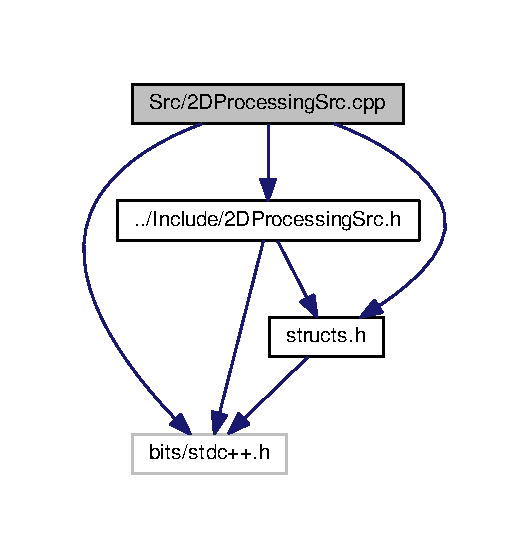
\includegraphics[width=254pt]{2DProcessingSrc_8cpp__incl}
\end{center}
\end{figure}

\hypertarget{3DProcessingSrc_8cpp}{}\section{3\+D\+Processing\+Src.cpp File Reference}
\label{3DProcessingSrc_8cpp}\index{3\+D\+Processing\+Src.\+cpp@{3\+D\+Processing\+Src.\+cpp}}
{\ttfamily \#include $<$bits/stdc++.\+h$>$}\\*
{\ttfamily \#include $<$structs.\+cpp$>$}\\*
Include dependency graph for 3\+D\+Processing\+Src.cpp\+:
% FIG 0
This graph shows which files directly or indirectly include this file\+:
% FIG 1
\subsection*{Classes}
\begin{DoxyCompactItemize}
\item 
class \hyperlink{classThreeDGraph__class}{Three\+D\+Graph\+\_\+class}
\begin{DoxyCompactList}\small\item\em 3D behaviour class. \end{DoxyCompactList}\end{DoxyCompactItemize}

\hypertarget{Index_8cpp}{}\section{Index.\+cpp File Reference}
\label{Index_8cpp}\index{Index.\+cpp@{Index.\+cpp}}
{\ttfamily \#include \char`\"{}cop/mainwindow.\+h\char`\"{}}\\*
{\ttfamily \#include $<$Q\+Application$>$}\\*
{\ttfamily \#include \char`\"{}bits/stdc++.\+h\char`\"{}}\\*
{\ttfamily \#include $<$Qt\+Core$>$}\\*
{\ttfamily \#include $<$Qt\+Gui$>$}\\*
{\ttfamily \#include $<$Q\+Label$>$}\\*
{\ttfamily \#include \char`\"{}structs.\+h\char`\"{}}\\*
{\ttfamily \#include \char`\"{}2\+D\+Processing\+Src.\+h\char`\"{}}\\*
{\ttfamily \#include \char`\"{}3\+D\+Processing\+Src.\+h\char`\"{}}\\*
{\ttfamily \#include \char`\"{}Input\+Src.\+h\char`\"{}}\\*
{\ttfamily \#include \char`\"{}Output\+Src.\+h\char`\"{}}\\*
{\ttfamily \#include \char`\"{}Interactive\+Src.\+h\char`\"{}}\\*
{\ttfamily \#include \char`\"{}mainwindow.\+h\char`\"{}}\\*
{\ttfamily \#include \char`\"{}ui\+\_\+mainwindow.\+h\char`\"{}}\\*
{\ttfamily \#include \char`\"{}dialog.\+h\char`\"{}}\\*
{\ttfamily \#include \char`\"{}ui\+\_\+dialog.\+h\char`\"{}}\\*
{\ttfamily \#include \char`\"{}interactiveinput.\+h\char`\"{}}\\*
{\ttfamily \#include \char`\"{}ui\+\_\+interactiveinput.\+h\char`\"{}}\\*
{\ttfamily \#include $<$Q\+File\+Dialog$>$}\\*
{\ttfamily \#include $<$Q\+Dir$>$}\\*
Include dependency graph for Index.\+cpp\+:
% FIG 0
\subsection*{Functions}
\begin{DoxyCompactItemize}
\item 
int \hyperlink{Index_8cpp_a0ddf1224851353fc92bfbff6f499fa97}{main} (int argc, char $\ast$argv\mbox{[}$\,$\mbox{]})
\end{DoxyCompactItemize}
\subsection*{Variables}
\begin{DoxyCompactItemize}
\item 
\hyperlink{classTwoDGraph__class}{Two\+D\+Graph\+\_\+class} {\bfseries input\+\_\+2d}\hypertarget{Index_8cpp_a7b422d961385be1621c787c7778593bb}{}\label{Index_8cpp_a7b422d961385be1621c787c7778593bb}

\item 
\hyperlink{classThreeDGraph__class}{Three\+D\+Graph\+\_\+class} {\bfseries input\+\_\+3d}\hypertarget{Index_8cpp_a594364b5a7f006d761aa9a8cfcb68ea2}{}\label{Index_8cpp_a594364b5a7f006d761aa9a8cfcb68ea2}

\item 
\hyperlink{classInteractive__editor}{Interactive\+\_\+editor} {\bfseries I1}\hypertarget{Index_8cpp_a403922218be213881144c168aac549c3}{}\label{Index_8cpp_a403922218be213881144c168aac549c3}

\item 
\hyperlink{classOutput}{Output} {\bfseries O1}\hypertarget{Index_8cpp_a74c85b6f0cd4748d25b91ba68d28b9be}{}\label{Index_8cpp_a74c85b6f0cd4748d25b91ba68d28b9be}

\item 
\hyperlink{classOutput}{Output} {\bfseries O2}\hypertarget{Index_8cpp_a805ab3302ab876a5f85457d063bf5bbd}{}\label{Index_8cpp_a805ab3302ab876a5f85457d063bf5bbd}

\item 
bool {\bfseries is\+File3d}\hypertarget{Index_8cpp_ab82efbeaa2890f39bf11e2ca4a83ce1b}{}\label{Index_8cpp_ab82efbeaa2890f39bf11e2ca4a83ce1b}

\item 
bool {\bfseries is\+Input\+File}\hypertarget{Index_8cpp_a82277de5e18d1e9caabbdeea50a0cd49}{}\label{Index_8cpp_a82277de5e18d1e9caabbdeea50a0cd49}

\item 
string {\bfseries filename}\hypertarget{Index_8cpp_a3a1a90139c2c8ab1fca0ea8b1790b7b2}{}\label{Index_8cpp_a3a1a90139c2c8ab1fca0ea8b1790b7b2}

\end{DoxyCompactItemize}


\subsection{Function Documentation}
\index{Index.\+cpp@{Index.\+cpp}!main@{main}}
\index{main@{main}!Index.\+cpp@{Index.\+cpp}}
\subsubsection[{\texorpdfstring{main(int argc, char $\ast$argv[])}{main(int argc, char *argv[])}}]{\setlength{\rightskip}{0pt plus 5cm}int main (
\begin{DoxyParamCaption}
\item[{int}]{argc, }
\item[{char $\ast$}]{argv\mbox{[}$\,$\mbox{]}}
\end{DoxyParamCaption}
)}\hypertarget{Index_8cpp_a0ddf1224851353fc92bfbff6f499fa97}{}\label{Index_8cpp_a0ddf1224851353fc92bfbff6f499fa97}
$<$ This is the orthographic projections 
\hypertarget{InputSrc_8cpp}{}\section{Input\+Src.\+cpp File Reference}
\label{InputSrc_8cpp}\index{Input\+Src.\+cpp@{Input\+Src.\+cpp}}
{\ttfamily \#include $<$bits/stdc++.\+h$>$}\\*
{\ttfamily \#include $<$Input\+Src.\+cpp$>$}\\*
{\ttfamily \#include $<$Output\+Src.\+cpp$>$}\\*
{\ttfamily \#include $<$2\+D\+Processing\+Src.\+cpp$>$}\\*
{\ttfamily \#include $<$3\+D\+Processing\+Src.\+cpp$>$}\\*
{\ttfamily \#include $<$Interactive\+Src.\+cpp$>$}\\*
Include dependency graph for Input\+Src.\+cpp\+:
% FIG 0
This graph shows which files directly or indirectly include this file\+:
% FIG 1
\subsection*{Classes}
\begin{DoxyCompactItemize}
\item 
class \hyperlink{classInput}{Input}
\begin{DoxyCompactList}\small\item\em \hyperlink{classInput}{Input} class. \end{DoxyCompactList}\end{DoxyCompactItemize}

\hypertarget{InteractiveSrc_8cpp}{}\section{Interactive\+Src.\+cpp File Reference}
\label{InteractiveSrc_8cpp}\index{Interactive\+Src.\+cpp@{Interactive\+Src.\+cpp}}
{\ttfamily \#include $<$bits/stdc++.\+h$>$}\\*
{\ttfamily \#include \char`\"{}structs.\+cpp\char`\"{}}\\*
{\ttfamily \#include \char`\"{}Graphs.\+cpp\char`\"{}}\\*
{\ttfamily \#include \char`\"{}Output\+Src.\+cpp\char`\"{}}\\*
{\ttfamily \#include \char`\"{}2\+D\+Processing\+Src.\+cpp\char`\"{}}\\*
{\ttfamily \#include \char`\"{}3\+D\+Processing\+Src.\+cpp\char`\"{}}\\*
Include dependency graph for Interactive\+Src.\+cpp\+:\nopagebreak
\begin{figure}[H]
\begin{center}
\leavevmode
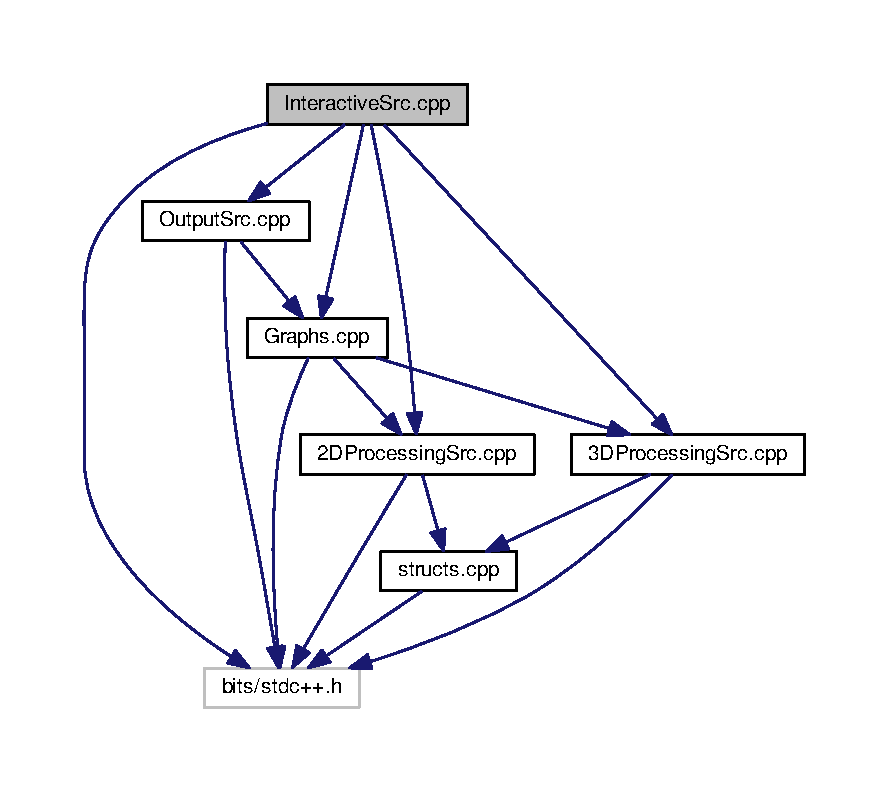
\includegraphics[width=350pt]{InteractiveSrc_8cpp__incl}
\end{center}
\end{figure}
This graph shows which files directly or indirectly include this file\+:\nopagebreak
\begin{figure}[H]
\begin{center}
\leavevmode
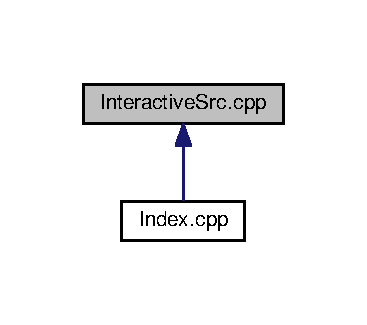
\includegraphics[width=176pt]{InteractiveSrc_8cpp__dep__incl}
\end{center}
\end{figure}
\subsection*{Classes}
\begin{DoxyCompactItemize}
\item 
class \hyperlink{classInteractive__editor}{Interactive\+\_\+editor}
\begin{DoxyCompactList}\small\item\em Editor class. \end{DoxyCompactList}\end{DoxyCompactItemize}

\hypertarget{OutputSrc_8cpp}{}\section{Output\+Src.\+cpp File Reference}
\label{OutputSrc_8cpp}\index{Output\+Src.\+cpp@{Output\+Src.\+cpp}}
{\ttfamily \#include $<$bits/stdc++.\+h$>$}\\*
{\ttfamily \#include $<$Input\+Src.\+cpp$>$}\\*
{\ttfamily \#include $<$Output\+Src.\+cpp$>$}\\*
{\ttfamily \#include $<$2\+D\+Processing\+Src.\+cpp$>$}\\*
{\ttfamily \#include $<$3\+D\+Processing\+Src.\+cpp$>$}\\*
{\ttfamily \#include $<$Interactive\+Src.\+cpp$>$}\\*
Include dependency graph for Output\+Src.\+cpp\+:
% FIG 0
This graph shows which files directly or indirectly include this file\+:
% FIG 1
\subsection*{Classes}
\begin{DoxyCompactItemize}
\item 
class \hyperlink{classOutput}{Output}
\begin{DoxyCompactList}\small\item\em Render and save class. \end{DoxyCompactList}\end{DoxyCompactItemize}

%--- End generated contents ---

% Index
\backmatter
\newpage
\phantomsection
\clearemptydoublepage
\addcontentsline{toc}{chapter}{Index}
\printindex

\end{document}
